\documentclass[12pt]{article}
\usepackage{amsmath}
\usepackage{multirow}
\usepackage{enumerate}
\usepackage{graphicx}
\usepackage{changepage}
\usepackage[all]{xy}
\usepackage{tikz}
\usetikzlibrary{shapes}
\usepackage{color}

\setlength{\voffset}{-3cm}
%\setlength{\hoffset}{-2cm}
%\setlength{\parindent}{0cm}
\setlength{\textheight}{26cm}
%\setlength{\textwidth}{14cm}
\newcommand{\tcr}{\textcolor{red}}

\begin{document}


\begin{center}
{\bf\Huge TEMPLATE EXAM\\[0.5cm]}
\quad\\[1cm]
\tcr{{\bf\large IMPORTANT NOTES\\[0.0cm]}}
\begin{itemize}
\item Topics {\bf NOT} on the final exam:
\begin{itemize}
\item Counting Techniques - Lecture5
\item Chi-Squared Test - Lecture17
\end{itemize}
\item Students who do well in the final exam will be graded as:
\begin{itemize}
\item Best midterm (15\%) + project (10\%) + final exam (75\%).\\
{\footnotesize(otherwise the original scheme stands: 30\% + 10\% + 60\%)}
\item Thus, you can still do very well in the module (even if the midterms didn't go your way).
\item In order to do well in the final exam, you must set everything out logically using correct symbols etc. (see points in red below).
\end{itemize}
\end{itemize}
\quad\\[1cm]
\begin{adjustwidth}{-1cm}{0cm}
\begin{tabular}{l@{\qquad}l}
MODULE CODE: MA4413&SEMESTER: Autumn 2014\\[1cm]
MODULE TITLE: Statistics for Computing& DURATION OF EXAM: 2.5 hours\\[1cm]
LECTURER: Dr.~Kevin Burke& GRADING SCHEME: 100 marks \\
& \hspace{3cm} (60\% of module)\\[2cm]
%EXTERNAL EXAMINER:&\\
%Prof. Brendan Murphy&\\[1cm]
\end{tabular}
\end{adjustwidth}
{\bf INSTRUCTIONS TO CANDIDATE}
\end{center}
\begin{small}
\begin{itemize}\itemsep0.3cm
\item {\bf Attempt four} of the six questions (each one carries 25 marks).
\item \tcr{All work must be shown \emph{clearly and logically} using appropriate symbols and probability notation. Failure to do so will \emph{lose marks}.}
\item \tcr{Write down the formula you intend to use at each stage \emph{before} filling it in with numbers.}
\item Formula sheets are provided at the back of this exam paper.
\item Statistical tables are available from the invigilators.
\end{itemize}
\end{small}
\newpage

\section*{Question 1 \qquad{\small(25 Marks)}}
\noindent\rule{\linewidth}{1pt}
\quad\\[-0.5cm]
\begin{enumerate}[a)]
\item {\bf Boxplots:}
\begin{itemize}
\item Lecture2 %Q3, Q4
\item Tutorial1 Q3, Q4(d)(e)(f)
\end{itemize}
\begin{center}\noindent\rule{0.4\linewidth}{0.5pt}\end{center}
\item {\bf Data types:}
\begin{itemize}
\item Lecture1 %Q3
\item Tutorial1 Q2
\end{itemize}
    \begin{center}\noindent\rule{0.4\linewidth}{0.5pt}\end{center}
\item {\bf Identify parameter \& statistic / calculate confidence interval:}
\begin{itemize}
\item Lecture1 %Q1, Q2
\item Lecture13
\item Tutorial1 Q1, Q2
\item Tutorial7 Q1, Q2, Q3, Q4, Q5
\end{itemize}
\end{enumerate}
\quad\\[-0.3cm]
\noindent\rule{\linewidth}{1pt}

\newpage

\section*{Question 2 \qquad{\small(25 Marks)}}
\noindent\rule{\linewidth}{1pt}
\quad\\[-0.5cm]
\begin{enumerate}[a)]
\item {\bf Histogram:}
\begin{itemize}
\item Lecture1 %Q5
\item Tutorial1 Q4
\item Lecture2-Q1
\end{itemize}
\begin{center}\noindent\rule{0.4\linewidth}{0.5pt}\end{center}
\item {\bf Inference concerning difference in means ($\mu_1-\mu_2$):}
\begin{itemize}
\item Lecture13
\item Lecture14 %Salary example (slides 18-29)
\item Lecture16 %CPU example (slides 12-19)
\item Tutorial7 Q5
\item Tutorial8 Q2
\item Tutorial10 Q1, Q2, Q3
\end{itemize}
\end{enumerate}
\quad\\[-0.3cm]
\noindent\rule{\linewidth}{1pt}

\newpage



\section*{Question 3 \qquad{\small(25 Marks)}}
\noindent\rule{\linewidth}{1pt}
\quad\\[-0.5cm]
\begin{enumerate}[a)]
\item {\bf Inference concerning one mean ($\mu$):}
\begin{itemize}
\item Lecture13
\item Lecture14 %Q1
\item Lecture15 %Q1, Q2
\item Tutorial7 Q2, Q3, Q6, Q7
\item Tutorial9 Q1, Q2, Q3, Q4
\end{itemize}
\begin{center}\noindent\rule{0.4\linewidth}{0.5pt}\end{center}
\item {\bf Basic probability rules:}
\begin{itemize}
\item Lecture3 %Q2, Q3, Q4
\item Lecture4 %Q1
\item Tutorial1 Q6, Q7
\end{itemize}
    \begin{center}\noindent\rule{0.4\linewidth}{0.5pt}\end{center}
\item {\bf Law of total probability:}
\begin{itemize}
\item Lecture4 %Q4
\item Tutorial2 Q2, Q3
\item Tutorial5 Q4
\item Tutorial6 Q2
\item Note: For the exam question you will be told that\\
\quad$\bullet\,\, X\,|\,A_1 \sim \text{Normal}(\mu_1,\sigma_1)$ and\\
\quad$\bullet\,\, X\,|\,A_2 \sim \text{Normal}(\mu_2,\sigma_2)$.\\
 $\Rightarrow$ $\Pr(X>x\,|\,A_1)$ and $\Pr(X>x\,|\,A_2)$ must be calculated using normal tables.
\end{itemize}
\end{enumerate}
\quad\\[-0.3cm]
\noindent\rule{\linewidth}{1pt}

\newpage




\section*{Question 4 \qquad{\small(25 Marks)}}
\noindent\rule{\linewidth}{1pt}
\quad\\[-0.5cm]
\begin{enumerate}[a)]
\item {\bf RAID:}
\begin{itemize}
\item Lecture3 Q3, Q5
\item Tutorial1 Q8
\item Note: When finding the number of cheap disks required to meet a desired failure probability, you must use $\log$s to solve.\\ (see Lecture3 Solutions ``Q5(e) - alternative method'')
\end{itemize}
\begin{center}\noindent\rule{0.4\linewidth}{0.5pt}\end{center}
\item {\bf Binomial:}
\begin{itemize}
\item Lecture7 %Q1, Q2
\item Tutorial3 Q4, Q5, Q6
\end{itemize}
    \begin{center}\noindent\rule{0.4\linewidth}{0.5pt}\end{center}
\item {\bf Poisson:}
\begin{itemize}
\item Lecture8 %Q2, Q3
\item Lecture9 (knowledge of exponential distribution is also needed)
\item Tutorial4 Q2
\end{itemize}
\end{enumerate}
\quad\\[-0.3cm]
\noindent\rule{\linewidth}{1pt}

\newpage




\section*{Question 5 \qquad{\small(25 Marks)}}
\noindent\rule{\linewidth}{1pt}
\quad\\[-0.5cm]
\begin{enumerate}[a)]
\item {\bf Random variable basics:}
\begin{itemize}
\item Lecture6 %Q1, Q2, Q3
\item Tutorial3 Q1, Q3(a)
\end{itemize}
\begin{center}\noindent\rule{0.4\linewidth}{0.5pt}\end{center}
\item {\bf Inference concerning one proportion ($p$):}
\begin{itemize}
\item Lecture13
\item Lecture15 %Q3
\item Tutorial7 Q1, Q4(d)
\item Tutorial9 Q5, Q6, Q7, Q8
\end{itemize}
    \begin{center}\noindent\rule{0.4\linewidth}{0.5pt}\end{center}
\item {\bf Normal distribution:}
\begin{itemize}
\item Lecture10 %Q2
\item Lecture12 %Q1
\item Tutorial5 Q5, Q6
\item Tutorial6 Q1(a)(b), Q3(c), Q4(a)(b)
\end{itemize}
\end{enumerate}
\quad\\[-0.3cm]
\noindent\rule{\linewidth}{1pt}

\newpage







\section*{Question 6 \qquad{\small(25 Marks)}}
\noindent\rule{\linewidth}{1pt}
\quad\\[-0.5cm]
\begin{enumerate}[a)]
\item {\bf Queueing theory:}
\begin{itemize}
\item Lecture9
\item Tutorial4 Q5, Q6, Q7
\item Tutorial5 Q1, Q2, Q3
\end{itemize}
\begin{center}\noindent\rule{0.4\linewidth}{0.5pt}\end{center}
\item {\bf Huffman coding:}
\begin{itemize}
\item Lecture18 %Q3
\item Tutorial11 Q1, Q2, Q3.
\end{itemize}
\end{enumerate}
\quad\\[-0.3cm]
\noindent\rule{\linewidth}{1pt}

\newpage














\section*{Useful Formulae: Page 1\\[0.3cm]}
{\bf Histogram:}\\[-0.8cm]
\begin{align*}
\bullet\quad \text{class width} = \frac{\max(x) - \min(x)}{\text{number of classes}}\\
\end{align*}
{\bf Numerical Summaries:}\\[-0.8cm]
\begin{align*}
\bullet\quad \bar x &= \frac{\sum\,x_i}{n}\\[0.6cm]
\bullet\quad s^2 &= \frac{\sum\,x_i^2 - n\,\bar x^2}{n-1}\\[0.6cm]
\bullet\quad \text{Position of } Q_k:& \quad \frac{n+1}{4}\times k \\[0.6cm]
\bullet\quad IQR &= Q_3 - Q_1 \\[0.6cm]
\bullet\quad LF &= Q_1 - 1.5 \times IQR \\[0.6cm]
\bullet\quad UF &= Q_3 + 1.5 \times IQR\\
\end{align*}
{\bf Probability:}\\[-0.8cm]
\begin{align*}
\bullet\quad \Pr(A^c) &= 1 - \Pr(A) \\[1cm]
\bullet\quad \Pr(A \cup B) &= \Pr(A) + \Pr(B) - \Pr(A \cap B)\\[0.6cm]
\bullet\quad \Pr(E_1 \cup E_2 \cup \cdots \cup E_k) &= \Pr(E_1) + \Pr(E_2) + \cdots + \Pr(E_k) \text{\quad{\footnotesize(if mutually exclusive)}}\\[1cm]
\bullet\quad \Pr(A \cap B) &= \Pr(A) \, \Pr(B \, | \, A) = \Pr(B) \, \Pr(A \, | \, B) \\[0.6cm]
\bullet\quad \Pr(E_1 \cap E_2 \cap \cdots \cap E_k) &= \Pr(E_1) \, \Pr(E_2) \, \cdots \, \Pr(E_k) \text{\quad{\footnotesize(if independent)}}\\[1cm]
\bullet\quad \Pr(A\,|\,B) &= \frac{\Pr(A \cap B)}{\Pr(B)} = \frac{\Pr(A) \,\Pr(B\,|\,A)}{\Pr(B)}\\[1cm]
\bullet\quad \Pr(B) = \Pr(B \cap E_1) &+ \Pr(B \cap E_2) + \cdots + \Pr(B \cap E_k) \\[0.2cm]
= \Pr(E_1) \, \Pr(B\,|\,&E_1) + \Pr(E_2) \, \Pr(B\,|\,E_2) + \cdots + \Pr(E_k) \, \Pr(B\,|\,E_k)\\[0.1cm]
\text{{\footnotesize(if $E_1,\ldots, E_k$}} & \,\, \text{{\footnotesize are mutually exclusive \& exhaustive)}}
\end{align*}

\newpage

\section*{Useful Formulae: Page 2\\[0.3cm]}
{\bf Counting Techniques:}\\[-0.8cm]
\begin{align*}
\bullet\quad n\,! &= n\times(n-1)\times(n-2)\times\cdots\times3\times2\times 1\\[0.6cm]
\bullet\quad \binom{n}{k} &= \frac{n\,!}{k\,! \,(n-k)\,!}\\
\end{align*}
{\bf Random Variables:}\\[-0.8cm]
\begin{align*}
\bullet\quad E(X) &= \sum x_i \,\, p(x_i)\\[0.6cm]
\bullet\quad E(X^2) &= \sum x_i^2 \,\, p(x_i)\\[0.6cm]
\bullet\quad Var(X) &= E(X^2) - [E(X)]^2\\[0.6cm]
\bullet\quad Sd(X) &= \sqrt{Var(X)}\\
\end{align*}
{\bf Distributions:}\\[-0.0cm]
\begin{adjustwidth}{-2.1cm}{0cm}
\begin{tabular}{|c@{\quad}|c@{\quad}|c@{\quad}|}
\hline
&&\\[-0.3cm]
$\bullet\quad X \sim \text{Binomial}(n,p)$ & $\bullet\quad X \sim \text{Poisson}(\lambda)$ & $\bullet\quad T \sim \text{Exponential}(\lambda)$ \\[0.6cm]
${\displaystyle\bullet\quad \Pr(X=x) = \binom{n}{x}\,p^x\,(1-p)^{n-x}}$ & ${\displaystyle\bullet\quad \Pr(X=x) = \frac{\lambda^x}{x\,!}\,\,e^{-\lambda}}$ & $\bullet\quad \Pr(T>t) = e^{-\lambda\,t}$ \\[0.8cm]
$\bullet\quad x \in \{0,1,2,\ldots,n\}$ & $\bullet\quad x \in \{0,1,2,\ldots,\infty\}$ & $\bullet\quad t \in [0,\,\infty)$ \\[0.8cm]
$\bullet\quad E(X) = n\,p$ & $\bullet\quad E(X) = \lambda$ & ${\displaystyle\bullet\quad E(T) = \frac{1}{\lambda}}$ \\[0.8cm]
$\bullet\quad Var(X) = n\,p\,(1-p)$ & $\bullet\quad Var(X) = \lambda$ & ${\displaystyle\bullet\quad Var(T) = \frac{1}{\lambda^2}}$ \\[0.4cm]
\hline
\multicolumn{3}{c}{}\\
\multicolumn{3}{c}{{\bf Note: the normal distribution is shown on the next page}}
\end{tabular}
\end{adjustwidth}




\newpage

\section*{Useful Formulae: Page 3\\[0.3cm]}
{\bf Queueing Theory:}\\[-0.8cm]
\begin{align*}
\bullet\quad E(N) &= \lambda_a\,E(T)\\[0.6cm]
\bullet\quad \rho &= \frac{\lambda_a}{\lambda_s}\\[0.6cm]
\xymatrixcolsep{0.5cm}
\bullet\quad M/M/1 \text{ System:} \quad & \xymatrix{\lambda_a \ar@{->}[r] & \hspace{-0.1cm}
{\begin{tabular}{@{}c|@{}c|@{}c|@{}c|@{}c|@{}c}
\cline{1-5}
&&&& &
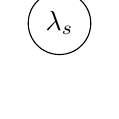
\begin{tikzpicture}[baseline=(char.base)]
\node(char)[draw,shape=circle]{$\lambda_s$};
\end{tikzpicture}\\
\cline{1-5}
\end{tabular}} \hspace{-0.3cm}\ar@{->}[r] &  \lambda_a} \\[0.6cm]
&\Rightarrow \,\, T \sim \text{Exponential}(\lambda_s-\lambda_a)\\[0.1cm]
{\footnotesize(\text{where $T$}} & {\footnotesize\text{ is the total time in the system)}}\\
\end{align*}

{\bf Normal Distribution:}\\[-0.6cm]
\begin{align*}
\bullet\quad X \sim \text{Normal}&(\mu,\sigma) \\[0.4cm]
\bullet\quad E(X) &= \mu \\[0.4cm]
\bullet\quad Var(X) &= \sigma^2 \\[0.4cm]
\bullet\quad (1-\alpha)100\% \text{ of the Normal}(\mu,\sigma) & \text{ distribution lies in } \mu \pm z_{\,\alpha/2}\,\,\sigma \\[0.4cm]
\bullet\quad \Pr(X > x) &= \Pr\left(Z> \frac{x-\mu}{\sigma}\right)\\[1cm]
\bullet\quad \Pr(Z < -z) &= \Pr(Z > z) \\[0.6cm]
\bullet\quad \Pr(Z > -z) &= \Pr(Z < z) = 1 -\Pr(Z>z) \\[1cm]
\bullet\quad \text{If} \,\,  X_1 \sim \text{Normal}(\mu_1,\sigma_1) \,\,  & \text{ and } \,\, X_2 \sim \text{Normal}(\mu_2,\sigma_2) \\[0.4cm]
\Rightarrow \quad  \text{ Sum: } \quad  X_1 + X_2 &\sim \text{Normal}\left(\mu_1+\mu_2,\,\sqrt{\sigma_1^2+\sigma_2^2}\,\right) \\[0.4cm]
\Rightarrow \quad  \text{ Difference: } \quad   X_1 - X_2 &\sim \text{Normal}\left(\mu_1-\mu_2,\,\sqrt{\sigma_1^2+\sigma_2^2}\,\right) \\[1cm]
\bullet\quad \text{For} \,\,  X_1,\ldots,X_n \sim \text{any distribution} & \text{ with } \mu = E(X) \text{ and } \sigma = Sd(X) = \sqrt{Var(X)}\\[0.4cm]
\Rightarrow \quad  \text{ Sample mean: } \quad  \,\overline{\!X} &\sim \text{Normal}\left(\mu,\,\frac{\sigma}{\sqrt{n}}\,\right) \quad \text{ if } n > 30
\end{align*}

\newpage


\section*{Useful Formulae: Page 4\\[0.3cm]}
{\bf Statistics and Standard Errors:}\\[0.1cm]
\begin{adjustwidth}{-2cm}{0cm}
\begin{tabular}{|c|c|c|c|c|}
\hline
&&&&\\[-0.1cm]
Parameter & Statistic & Standard Error & Samples & Details \\[0.3cm]
\hline
&&&&\\[-0.1cm]
$\mu$ & $\bar x$ & ${\displaystyle\frac{s}{\sqrt{n}}}$  & large / small & $\nu = n - 1$ \\[0.5cm]
\hline
&&&&\\[-0.1cm]
$p$ & $\hat p$ & \multirow{2}{*}{${\displaystyle\sqrt{\frac{\hat p\,(1-\hat p)}{n}}}$} & large & confidence \\[-0.1cm]
&&&&interval\\[0.3cm]
\cline{3-5}
&&&&\\[-0.1cm]
&  & \multirow{2}{*}{${\displaystyle\sqrt{\frac{p_0\,(1-p_0)}{n}}}$} & large & hypothesis \\[-0.1cm]
&&&&test\\[0.3cm]
\hline
&&&&\\[-0.1cm]
$\mu_1-\mu_2$ & $\bar x_1 - \bar x_2$ & \multirow{3}{*}{${\displaystyle\sqrt{\frac{s_1^2}{n_1}+\frac{s_2^2}{n_2}}}$} & large / small & ${\displaystyle \nu = \frac{(a+b)^2}{\frac{a^2}{n_1-1}+\frac{b^2}{n_2-1}}}$ \\[0.8cm]
&&&& ${\displaystyle a=\frac{s_1^2}{n_1}, \,\,\, b=\frac{s_2^2}{n_2}}$ \\[0.5cm]
\cline{3-5}
&&&&\\[-0.1cm]
&  & ${\displaystyle\sqrt{\frac{s_p^2}{n_1}+\frac{s_p^2}{n_2}}}$ & small & $\nu = n_1+n_2-2$ \\[0.5cm]
&&&& assuming \\[-0.2cm]
&& where\,\, ${\displaystyle s_p^2 = \frac{(n_1-1)\,s_1^2+(n_2-1)\,s_2^2}{n_1+n_2-2}}$  && $\sigma_1^2 = \sigma_2^2$ \\[0.5cm]
\hline
&&&&\\[-0.1cm]
$p_1-p_2$ & $\hat p_1 - \hat p_2$ & \multirow{2}{*}{${\displaystyle\sqrt{\frac{\hat p_1 \, (1-\hat p_1)}{n_1}+\frac{\hat p_2 \, (1-\hat p_2)}{n_2}}}$} & large & confidence\\[-0.1cm]
&&&&interval\\[0.5cm]
\cline{3-5}
&&&&\\[-0.1cm]
&  & ${\displaystyle\sqrt{\frac{\hat p_c\,(1-\hat p_c)}{n_1}+\frac{\hat p_c\,(1-\hat p_c)}{n_2}}}$ & large & hypothesis\\[-0.4cm]
&&&&test\\[0.2cm]
&&where\,\, ${\displaystyle \hat p_c = \frac{x_1+x_2}{n_1+n_2}}$&&\\[0.5cm]
\hline
\multicolumn{5}{c}{}\\[0.5cm]
\end{tabular}
\end{adjustwidth}
{\bf Confidence Intervals:}\\[-0.5cm]
\begin{align*}
\bullet\quad \text{Large sample:} \qquad \text{statistic } &\pm\,\, z_{\,\alpha/2}\,\times\,\text{standard error} \\[0.6cm]
\bullet\quad \text{Small sample:} \qquad \text{statistic } &\pm\,\, t_{\,\nu,\,\alpha/2}\,\times\,\text{standard error}
\end{align*}

\newpage

\section*{Useful Formulae: Page 5\\[0.3cm]}
{\bf Hypothesis Testing:}\\[-0.5cm]
\begin{align*}
\bullet\quad z &= \frac{\text{statistic}-\text{hypothesised value}}{\text{standard error}} \\[1cm]
\bullet\quad \text{p-value } &= \left\{
\begin{array}{rl}
2 \times \Pr(Z > |z|) & \text{if }  H_a: \, \mu \ne \mu_0\\[0.4cm]
\Pr(Z < z) & \text{if } H_a: \, \mu < \mu_0\\[0.4cm]
\Pr(Z > z) & \text{if } H_a: \, \mu > \mu_0\\
\end{array} \right.\\[1cm]
\bullet\quad F &= \frac{\text{larger variance}}{\text{smaller variance}} = \frac{s_{\text{larger}}^2}{s_{\text{smaller}}^2} \\[0.5cm]
 & \nu_1 = n_{\text{\,top}} - 1,\quad\, \nu_2 = n_{\text{\,bottom}} - 1 \\[1cm]
\bullet\quad \chi^2 &= \sum \frac{(o_i-e_i)^2}{e_i}\\[0.5cm]
\text{Goodness-of-fit: } \qquad &e_i = \text{total} \times p(x_i),\qquad \nu = n_f - 1- k \\[0.6cm]
\text{Independence: } \qquad &e_{ij} = \frac{r_i\,\times\,c_j}{\text{total}},\qquad \nu = (n_r - 1)\,\times\,(n_c - 1)\\[0.3cm]
\end{align*}
{\bf Information Theory:}\\[-0.5cm]
\begin{align*}
\bullet\quad h(x) &= - \log_2[p(x)] \\[0.6cm]
\bullet\quad H(X) &= E[h(X)] = \sum h(x_i)\,p(x_i) \\[1cm]
\bullet\quad l(x_i) &= \text{code-length for character } x_i \\[0.6cm]
\bullet\quad E(L) &= \sum l(x_i)\,p(x_i) \\[1cm]
\bullet\quad e &= \frac{H(X)}{E(L)} \\[1cm]
\bullet\quad &\sum 2^{-l(x_i)}  \le 1
\end{align*}


\end{document} 